\StartOf{Lecture 20}

\Today{(1) MIMO, (2) Wi-Fi protocol}

\announcements{
\begin{itemize}
  \item Homework 9 due Wed at 11:59pm.
  \item Exam 2 is Mon April 20.  Schedule 80 minutes of your day to take this exam.  Most should take it during the class period, but if your schedule / time zone makes this difficult you may pick a different 80 minute period.
\end{itemize}
}


\section{MIMO}

Multiple-input multiple output (MIMO) is a particular type of space and/or polarization diversity in which both the transmitter and receiver may use multiple antennas.  

\begin{figure}[htbp]
\centerline{ 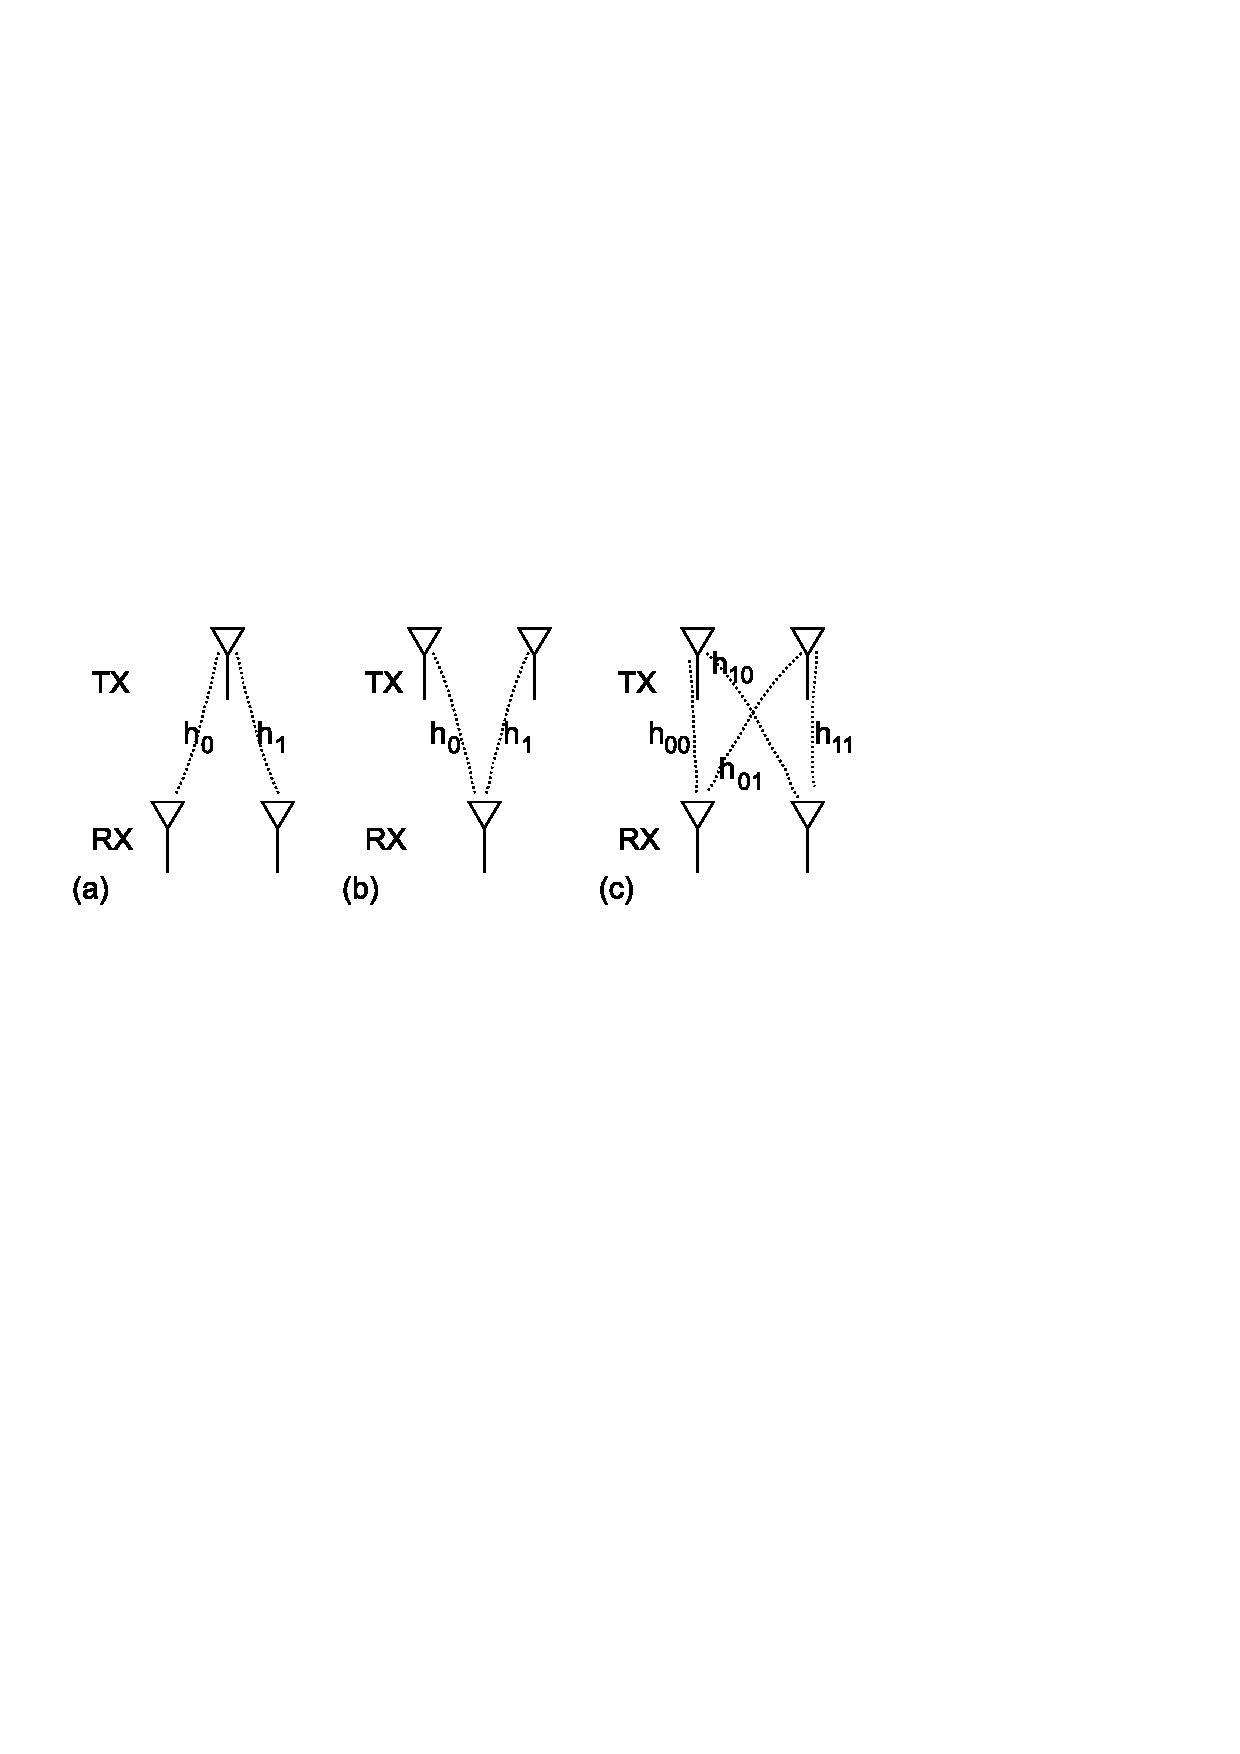
\includegraphics[width=4in]{images/mrc_and_mimo.png} }
\caption{Transmit and receive space diversity schemes: (a) traditional space diversity with receiver combining, called single input multiple output (SIMO); (b) transmit diversity, which may use Alamouti's scheme, called multiple input single output (MISO); (c) $2\times 2$ multiple input multiple output (MIMO).}
    \label{F:mrc_and_mimo}
\end{figure}

To introduce the topic, I need to discuss multipath fading.  Multipath is the phenomenon that multiple waves, each arriving from different directions, arrives at the receiver antenna, and the voltage measured at the receiver is a phasor sum of the complex amplitudes of these waves. The phases of these waves change as the antenna moves, but each wave's rate of phase change is different, depending on its angle of arrival. Thus as the phases change at different rates, the phasor sum of the waves change with respect to each other.  Sometimes, the complex amplitudes with have similar phases and add constructively.  Other times, these complex amplitudes are nearly opposite in phase, and when added, are at or near the origin.     The effect of multipath fading on the received power (the squared distance from the origin of the phasor sum of the complex amplitudes) is that it varies from a few dB gain to a 30 dB loss as the antenna moves on the order of a quarter of a wavelength.  This is a very severe problem for mobile communications since link budgets are tight (as you have seen) and there is not generally 30 dB to spare to make the link reliable even when fading is at its worst. 

The use of multiple antennas has been a standard technique in wireless communication to deal with multipath fading.  The idea, up until 20 years ago, was as shown in Figure \ref{F:mrc_and_mimo}(a), where one transmit antenna sent power to multiple receive antennas.  The receiver would use \emph{combining} to, for example, pick the receive antenna with the highest power (\textit{selection combining}), or multiply each received voltage with an optimal complex amplitude and add them together (\textit{maximal ratio combining}, or MRC), as introduced in the next section.

The use of multiple antennas is called \textit{space or polarization diversity}.  As the two antennas are separated in space (and can be differently polarized), their received powers are different realizations of random variables, and the receiver essentially can benefit from getting multiple ``chances'' at a good result, just like asking people with diverse opinions can increase your chances that someone helps you out.




\subsection{ Maximal Ratio Combining}

We're going to introduce MIMO by starting with maximal ratio combining (MRC). Let's assume that the transmitter sends symbol (complex) voltage $s$ out of its single antenna.  Assume the channel from TX to RX antenna 0 experiences total channel power gain $|h_0|^2$ (or voltage gain $h_0$), and the channel from TX to RX antenna 1 experiences total channel power gain $|h_1|^2$ (or voltage gain $h_1$).  That is, the two received voltages are
\begin{eqnarray} \label{E:TX_Signal}
 r_0 &=& h_0 s + n_0 \nnn
 r_1 &=& h_1 s + n_1 
\end{eqnarray}

In MRC, the received signals $r_0$ and $r_1$ are multiplied by higher values if the SNR is higher, and lower value, and then summed.  Multiplying received signals by a constant doesn't help (it amplifies the noise as much as the signal) so it really matters to multiply them by different numbers.  Here, those numbers turn out to be $h_0^*$ and $h_1^*$, that is, the complex conjugate of the channel gains.  In other words,
\[
 r_{MRC} = h_0^* r_0 + h_1^* r_1 
\]
That is,
\[
 r_{MRC} = \left[ |h_0|^2 + |h_1|^2 \right] s + h_0^* n_0 + h_1^* n_1
\]
In the case when we had only one receive antenna, we would have received either $r_1$ or $r_0$.  In comparison, the noise terms are multiplied by $h_0^*$ or $h_1^*$, but the signal is multiplied by the sum of $|h_0|^2 + h_1^2$.  If one $\alpha_i$ fades, we don't lose the entire signal $s$.

However, MRC requires exactly one transmit antenna, it is not a method to have multiple transmit antennas.

\subsection{Alamouti code}

MIMO started gaining steam in 1998, from two different results, one from Bell Labs, where they had built an experimental MIMO system they called V-BLAST \cite{wolniansky1998vblast}, and a simple transmit diversity scheme from S.\ M.\ Alamouti now called the Alamouti scheme \cite{alamouti1998simple}.  The Alamouti scheme is a simple way to achieve a performance similar to MRC using two transmit antennas, and a single receiver, like the system shown in Figure \ref{F:mrc_and_mimo}(b).  The advantage is that in some cases, the transmitter is more able to have multiple antennas, while the receiver is more limited in size (for example, cellular communications on the downlink).  

Alamouti presented a simple scheme that sends two symbols simultaneously, but takes two symbol periods to do so, and over the two transmit antennas.  Denote these two symbols $s_0$ and $s_1$.  The idea is, first transmit $s_0$ out of antenna 0 and $s_1$ out of antenna 1.  At the receiver, assuming the channels are $h_0$ and $h_1$, will be
\begin{equation} \label{E:r0}
r_0 = s_0 h_0  + s_1 h_1 
\end{equation}
Then, during the subsequent symbol period, send $-s_1^*$ out of antenna 0 and $s_0^*$ out of antenna 1, where the superscript $*$ is used to denote complex conjugate.  During the second symbol period the receiver will see
\begin{equation}\label{E:r1}
r_1 = -s_1^* h_0  + s_0^* h_1 
\end{equation}
Note this assumes the channel gains were the same during the second symbol period as during the first.

The ``magic'' happens when we combine $r_0$ and $r_1$ in the following way to come up with estimates of $s_0$ and $s_1$.  We form:
\begin{eqnarray}
\tilde{s}_0 &=& h_0^* r_0 + h_1 r_1^* \nnn
\tilde{s}_1 &=& h_1^* r_0 - h_0 r_1^* \nn
\end{eqnarray}
Plugging in for $r_0$ and $r_1$ as given in (\ref{E:r0}) and (\ref{E:r1}), respectively,
\begin{eqnarray}
\tilde{s}_0 &=& h_0^* (s_0 h_0 + s_1 h_1) + h_1 (-s_1 h_0^*  + s_0 h_1^* ) \nnn
\tilde{s}_1 &=& h_1^* (s_0 h_0  + s_1 h_1) - h_0  (-s_1 h_0^*  + s_0 h_1^*) \nn
\end{eqnarray}
Simplifying,
\begin{eqnarray}
\tilde{s}_0 &=& |h_0|^2 s_0 + s_1 h_0^* h_1  -s_1 h_0^* h_1  + |h_1|^2 s_0  \nnn
\tilde{s}_1 &=& |h_1|^2 s_1 + s_0 h_0 h_1^*  - s_0 h_0 h_1^*  + |h_0|^2 s_1  \nn
\end{eqnarray}
The middle terms cancel out in each case, so finally,
\begin{eqnarray}
\tilde{s}_0 &=& (|h_0|^2 + |h_1|^2) s_0  \nnn
\tilde{s}_1 &=& (|h_1|^2 + |h_0|^2) s_1  \nn
\end{eqnarray}
In short, in two symbol periods, we've managed to convey two symbols of information.  Each symbol arrives with approximately the same signal amplitude that we would have had in the maximal ratio combining case.

Notes:  
\begin{enumerate}
%
\item This is a two-by one code, that is, it works for two transmit antennas and one receive antenna.  This code has been generalized for $n\times m$ MIMO systems, and called ``space-time block codes'', by Tarokh et.~al.~\cite{tarokh1999space}.  These can send more symbols in less time -- in $k$ symbol periods, you can send more than $k$ symbols.
%
\item If you transmit out of two antennas, you would in general need twice as much power as the receiver diversity case, which had one transmit antenna.  So generally we compare the two when using the same total transmit power, \ie, cut the power in half in the transmitter diversity case.  The performance is thus 3 dB worse than the receiver MRC diversity case.
%
\item The Alamouti and space-time block codes are not optimal.  Space-time coding is the name of the general area of encoding information the multiple channels.  One better-performing scheme is called space-time trellis coding.  But the decoding complexity of space-time trellis codes increases exponentially as a function of the spectral efficiency \cite[p377]{haykin2005modern} \cite{tarokh1999space}.
%
\end{enumerate}


\subsection{MIMO Channel Representation}

In general for MIMO, we have multiple ($N_t$) transmitters and multiple ($N_r$) receivers.  We refer to the system as a $(N_t,N_r)$ or $N_t \times N_r$ MIMO system.  Figure \ref{F:mrc_and_mimo}(c) shows the channels for a $(2,2)$ MIMO system.  For the channel between transmitter $k$ and receiver $i$, we denote the ``channel voltage gain'' as $h_{i,k}$.  This gain is a complex number, with real and imaginary parts.  Recall that the phase of a multipath component changes with distance, frequency, due to reflections, etc.  The channel power gain would be $|h_{i,k}|^2$. The received voltage signal at $i$, just from transmitter $k$, is $s_k h_{i,k}$, where $s_k$ is what was transmitted from antenna $k$.  

To keep all these numbers organized, we use vectors and matrices.  The transmitted signal from antennas $1, \ldots, N_t$ is denoted $\mbs$, 
\[
\mbs = [s_1, \ldots, s_{N_t}]^T
\]
and the channel gain matrix $H$ is given as
\begin{equation} \label{E:H}
H = \MatFourCols{
   h_{1,1} & h_{2,1} & \cdots & h_{N_t,1} \\
   h_{1,2} & h_{2,2} & \cdots & h_{N_t,2} \\
   \vdots & \vdots &  \ddots & \vdots \\
   h_{1,N_r} & h_{2,N_r} & \cdots & h_{N_t,N_r} \\
}
\end{equation}
Where there are $N_r$ rows each corresponding to the channels measured at each receiver; and $N_t$ columns each corresponding to the channels from each transmitter.

The received signal at receiver $i$ is a linear combination of the $s_k$ for $k=1,\ldots ,N_t$ terms plus noise:
\[
x_i = \sum_{k=1}^{N_t} h_{i,k} s_k + w_i
\]
where $w_i$ the additive noise term, and $i=1, \ldots, N_r$.  In matrix form, we can rewrite this as:
\[
\mbx = H \mbs + \mbw
\]
where $\mbx = [x_1, \ldots, x_{N_r}]^T$ is the received vector and $\mbw = [w_1, \ldots, w_{N_r}]^T$ is the noise vector.



\subsection{Capacity of MIMO Systems}

We said in the lecture on Shannon channel capacity  that there is a theoretical limit to the bps per Hz we can achieve on a channel.  Using multiple antennas at the TX and RX increases this theoretical limit.  We said that the limit on bandwidth efficiency is given as,
\begin{equation} \label{E:SISO_Shannon}
 \frac{R_{max}}{B} =  \log_2 \left( 1 + \rho \right)
\end{equation}
where $R_{max}$ is the maximum possible bit rate which can be achieved on the channel for given signal to noise ratio $\rho$ and bandwidth $B$.

In a $N_t \times N_r$ MIMO system with channel matrix $H$ as given in (\ref{E:H}), with $N_t \ge N_r$, the new Shannon limit on bps per Hz is \cite{haykin2005modern},
\begin{equation} \label{E:MIMO_Shannon_1}
 \frac{R_{max}}{B} =  \E{}{\log_2 \left\{ \mbox{det} \left( \I{N_r} + \rho\frac{1}{N_t} HH^\dagger \right) \right\} }
\end{equation}
where $H^\dagger$ is the complex conjugate of $H$ (I'm copying the notation of the Haykin Moher book), and $\rho$ is the average signal to noise ratio.  Here, we assume that each channel is Rayleigh, that is each channel voltage gain $h_{i,k}$ is complex Gaussian, and all channel gains are independent from each other.  This is why we need an expected value -- the matrix $H$ is filled with random variables. 

To get more intuition about the bandwidth efficiency limit, consider that the term $HH^\dagger$ 
is a Hermitian $N_r \times N_r$ matrix 
with eigendecomposition $H H^\dagger = U \Lambda U^\dagger$ 
where $U$ is the matrix of eigenvectors of $H H^\dagger$ and $\Lambda$ is a diagonal matrix of eigenvalues $\lambda_i$ for $i=1, \ldots, N_r$.  In this case, we can rewrite (\ref{E:MIMO_Shannon_1}) as,
\begin{equation} \label{E:MIMO_Shannon_2}
 \frac{R_{max}}{B} =  \E{}{\sum_{i=1}^{N_r} \log_2 \left( 1 + \rho \frac{\lambda_i}{N_t} \right)  }
\end{equation}
Compared to (\ref{E:SISO_Shannon}), Equation (\ref{E:MIMO_Shannon_2}) is a sum of several Shannon capacities -- each with effective SNR $\rho\frac{\lambda_i}{N_t}$.  Recall this was the formula for $N_t \ge N_r$.  For $N_r \ge N_t$, the formula is
\begin{equation} \label{E:MIMO_Shannon_3}
 \frac{R_{max}}{B} =  \sum_{i=1}^{N_t} \E{}{ \log_2 \left( 1 + \rho\frac{\lambda_i}{N_r} \right)  }
\end{equation}
These $\min (N_t, N_r)$ ``channels'' are called the ``eigen-mode channels'' of a MIMO system.

In summary, we have created $\min (N_t, N_r)$ eigen-mode channels.  Results have shown that the total capacity increases approximately with $\min (N_t, N_r)$.  MIMO is so attractive for current and future communication systems because it multiplies the achievable bit rate by this factor of $\min (N_t, N_r)$, without requiring additional bandwidth or signal energy.

% Key points
% 1.  The channel between multiple TX/RX antennas forms a complex matrix H
% 2.  The Shannon channel capacity can be increased using multiple antennas.  
%    a.  Can be written using HH^*
%    b.  Can be written using eigenvalues of H
% 3.  Space-time coding is a general way to encode information on the multiple channels.  Eg., space-time trellis codes.  But ``the decoding complexity of space-time trellis codes increases exponentially as a function of the spectral efficiency'' \cite[p377]{haykin2005modern}.
% 4.  Alamouti scheme is a suboptimal two-by-one MIMO space-time code
% 5.  Tarokh et. al. generalized this to arbitrary numbers of antennas for ``space-time block codes''.



\section{Wi-Fi: Example Protocols}

As an example wireless protocol we will consider 802.11 protocols advertised as \emph{Wi-Fi}. These are standardized by the IEEE, within its networking standards committee (802) for wireless local area networking (subcommittee \#11).  The protocols are all half-duplex, operating on the same frequency channel for both directions between two devices (commonly referred to as uplink, or to the access point, and downlink, or to the mobile device).  

\subsection{DS-SS}

The first (popular) protocol was called 802.11b, meant to operate in the 2.4 GHz ISM band in the US (2.400 to 2.483 GHz).  Prior to this protocol, most wireless devices operated below 1 GHz, for example, in the 902-928 MHz band.  The higher frequency band was a poor choice first because of its higher attenuation through walls, relatively higher cost of transceivers, and the microwave oven problem: microwave ovens had been allocated this same band.  Microwave ovens were thought to impose a nearly insurmountable robustness challenge, and the FCC couldn't sell the band to any paying customer, so they essentially were forced to ``give it away'' for free as a very large unregulated band.  To deal with the interference produced by microwave ovens, and other interfering ISM band transmissions, they specified that devices would have to use ``spread spectrum'' modulation methods.  Essentially, a transmitter must spread its signal across a very wide bandwidth in order to ``average out'' the effects of narrowband interfering signals.  

IEEE 802.11b met this requirement in a couple of different ways.  The first way is called \emph{direct sequence spread spectrum} (DS-SS).  In DS-SS, the pulse shape is artificially set to have a high bandwidth.  The 802.11b standard used what is called a \emph{Barker code} as its pulse shape.  The pulse shape $p(t)$ for the Barker code pulse shape is shown in Fig.~\ref{F:Barkercode} \cite{maas2012channel}.  The Barker code pulse shape is essentially the function you'd get by modulating (via binary bipolar PAM) the bits 10110111000 using a SRRC pulse.  These eleven ``fake bits'' used to generate the Barker code are called \emph{chips}. The Barker code pulse shape is wide in bandwidth; the symbol rate is 1 MSymbol/sec and the bandwidth of the signal is 11 times this because it is just like the bandwidth of a 11 Msymbol/sec BPSK signal with a  SRRC pulse shape (with a large $\alpha$).  

\begin{figure}[htbp]
  \centerline{\includegraphics[width=3.0in]{../images/Barker_v2-eps-converted-to.pdf}}
  \caption{Samples of the Barker code used in IEEE 802.11b \cite{maas2012channel}.}
  \label{F:Barkercode}
\end{figure}

The advantage of the Barker code is that it is nearly orthogonal to itself at non-zero delays.  If a correlator is running, it will see a sharp correlation peak when it is lined up perfectly with the incoming Barker code, and will be nearly zero when it is not.  This can help with symbol synchronization.  

The original two modulations for 802.11b are differential BPSK or differential QPSK.  We covered D-BPSK, but not D-QPSK.  D-QPSK is $M=4$ thus 2 bits per symbol, for a total of 2 Mbps, while D-BPSK has 1 Mbps.  If the link quality was high enough, the link would use D-QPSK.  

%There were two optional higher rate modulations added later for 802.11b, but they were not widely implemented, as far as I know.  They removed the Barker code, and essentially gave options for combinations of other orthogonal codes.

\subsection{OFDM}

The next major advancement was for 802.11g.  While 802.11a technically was released about the same time as 802.11b, the ``a'' standard specified using the 5.8 GHz band.  The combination of the computational costs of OFDM and the higher costs of 5.8 GHz components made for little commercial use initially.  IEEE 802.11g used the 2.4 GHz band for the same OFDM modulation, and thus was less expensive than ``a''.  OFDM, as we've described, uses many, many orthogonal sine and cosine waveforms, each at a different frequency.  Each sine and cosine pair at one frequency is called a subcarrier, and there are 52 subcarriers.  Four are sent un-modulated, that is with no data, just the sine or cosine wave itself, so that the receiver can perform synchronization.

The other 48 subcarriers in the OFDM signal are modulated with one of: BPSK, QPSK, 16 square QAM, or 64 square QAM.  For each there is a choice of two convolutional codes, the first which sends out two coded bits for each information bit input, that is, a rate 1/2 code; or 2) a code that sends out four coded bits for each three information bits input, that is, a rate 3/4 code.  You can see that the rate 3/4 code is more efficient, but it also corrects fewer errors.  In all, there are 8 modulation/coding schemes (MCS).  These are chosen adaptively, and communicated between devices so that the receiver knows what detector to use on each subcarrier.

The symbol rate in 802.11g is 4 $\mu$s.  However, 0.8 $\mu$s  of that symbol duration does not provide information; it simply repeats the final 0.8 $\mu$s at the beginning of the symbol.  It is called the \emph{cyclic prefix} and is used to make the symbol periodic.  Because of this periodicity, the IFFT and FFT can be successfully used to generate the temporal signal to transmit, and to separate the 52 subcarriers at the receiver.  Thus 3.2 $\mu$s of the symbol contains information.  However, each symbol contains 48 subcarriers, each with up to 6 bits (when using $M=64$ QAM, for a total of 288 bits per symbol. The maximum bit rate for 802.11g is this 288 coded bits per 4 $\mu$s, or at most $288(3/4)$ information bits per 4 $\mu$s, or 54 Mbps.  

\subsection{MIMO}

The next big development was the addition of multiple input multiple output (MIMO) methods to the standard.  IEEE 802.11n was the first major standardization of MIMO technology, which had just really been invented 9-10 years prior \cite{alamouti1998simple}.  By using $N$ antennas at the transmitter, and $N$ at the receiver, the idea of MIMO is to achieve $N$ ``separate'' spatial streams.  The 802.11n standard specified a maximum of $N=4$ at both end of the link, that is, $N_t = N_r = 4$ is the maximum.  The capacity is, theoretically, able to be multiplied by $\min (N_t, N_r) = 4$ at most.

%How?  Well, consider the radio channel on one subcarrier.  The channel between transmit antenna $i$ and receive antenna $j$ acts like a multiplication by a complex-value $h_{i,j}$.  Let's say I'm sending voltage $s_i$ out of antenna $i$ at a particular time.  So the received signal $r_j = h_{i,j} s_i$.  The channel is really linear, so if I send voltage $s_1$ through $s_N$ from each of my $N$ transmit antennas, then I'll receive 
%\[
%r_j = h_{1,j} s_1 + \cdots + h_{N,j} s_N
%\]
%at receive antenna $j$.  This is true for $j=1, \ldots, N$.  So lining up all $N$ equations in a matrix form, we can write
%\[
%\mbr = H \mbs,
%\]
%where $\mbr = [r_1, \ldots, r_N]^T$, $\mbs = [s_1, \ldots, s_N]^T$, and $H = [[ h_{i,j} ]]$ is an $N$ by $N$ matrix of the channel values.  Essentially, the goal of the MIMO receiver is, given the measurements $\mbr$, to compute the values of $\mbs$ as they were sent by multiplying both sides by some kind of inverse of $H$,
%\[
%H^{-1} \mbr = H^{-1} H \mbs = \mbs
%\]
%which results in us obtaining the original $N$ voltages originally sent.  Now, two things I've totally skipped over:
%\begin{enumerate}
%    \item We really really need to know the $H$ in order to be able to find its inverse, and
%    \item How do we know that the channel $H$ even \emph{has} an inverse?  
%\end{enumerate}
%These two complications are, well, quite complicated.  But generally speaking:
%\begin{enumerate}
%    \item The channel matrix $H$ is the same when the role of transmitter and receiver are reversed, as they are in a half-duplex time division duplex system like 802.11.  Thus the channel can be measured in one direction, and then used in the other direction.  
%    \item A matrix of Gaussian random complex numbers tends to be invertible.  Essentially, there needs to be enough  multipath from different directions to make the $H$ matrix invertible.  For large enough $N$, it won't be. 
%\end{enumerate}

The next generations of Wi-Fi use more antennas (up to 8 in 802.11ax), higher bandwidths (80 MHz), higher $M$ (up to 1024-QAM in 802.11ax) and mm-wave bands (60 GHz bands in 802.11ay).  The 60 GHz band is also an unlicensed band, and considerable bandwidth is available.   The band has been avoided for long range applications because it has about 10 dB loss / km due to oxygen (O$_2$) absorption.  There is 14 GHz of bandwidth available in this band.  The 802.11ay standard allows allocating 8 GHz for a single link.  One can achieve very high data rate with such a large bandwidth, even with modulations with low bandwidth efficiency.  



\subsection{Shortcomings}

One of the problems with Wi-Fi is range.  There is no rate lower than 1 Mbps, thus it is designed for relatively short range links. Recall that, for a given probability of bit error, you need a certain $\Ebno$.  The noise power spectral density $N_0$ is fixed; and $\En_b$ is the received power times the bit period, $T_b P_r$.  If you want to extend the range, the $P_r$ will go down, and you will be forced to increase the $T_b$, or equivalently, reduce the bit rate $R_b$.  Thus there is a tradeoff between range and data rate.  For many Internet-of-things (IoT) applications, the required data rate is very low compared to 1 Mbps.  For example, an air quality sensor might need to send a 50 bytes of air quality data per hour, or about 0.1 bps, seven orders of magnitude less than Wi-Fi's minimum rate.  

My lab has done some work to address the range limitation of Wi-Fi.  We created a protocol that one can run on top of Wi-Fi with a standard Wi-Fi transceiver, with a change in software, that enables a new very low rate but much longer range data communications.  It's called ``on-off noise communication'', and effectively uses regular Wi-Fi packets as a means to increase the interference in the channel \cite{lundrigan2019onpc}.  Even when those packets can't be demodulated because the transmitter is too far away, they increase the noise+interference power measured by a receiver.  Our protocol transmits and receives temporal patterns in the Wi-Fi noise level and uses them to send bits.  

Another problem with Wi-Fi for IoT is that the transceiver is relatively high in power consumption.  OFDM requires a linear amplifier, and relatively high transmit power.  Thus a transmission requires considerable power consumption.  Further computational complexity, multiple antennas, and the fact that the receiver spends considerable time constantly listening to the channel, means that the receiver consumes considerable energy as well.  For example, a 802.11n receiver can consume more than 1 W while in idle receive mode \cite{halperin2010demystifying}.   Prior to 802.11ah and ax, receivers were not permitted long sleep periods.  The addition of the \emph{target wake time} (TWT) provides a means for Wi-Fi endpoints (devices besides the access point) to sleep for a designated period of time.   Battery-powered low rate devices may prefer a modulation capable of more energy efficient operation.  


